\begin{frame}{Recurrent Neural Network}
    Advantages of using RNNs to model distortion circuits:
    \vspace{1ex}
    \begin{itemize}
        \itemsep0.5em
        \item Makes sense (recurrent units can be distortion effects)
        \item Computationally efficient
        \item Can include circuit control parameters
    \end{itemize}
\end{frame}

\begin{frame}{Recurrent Neural Network}
    \vspace{1ex}
    \begin{figure}
        \centering
        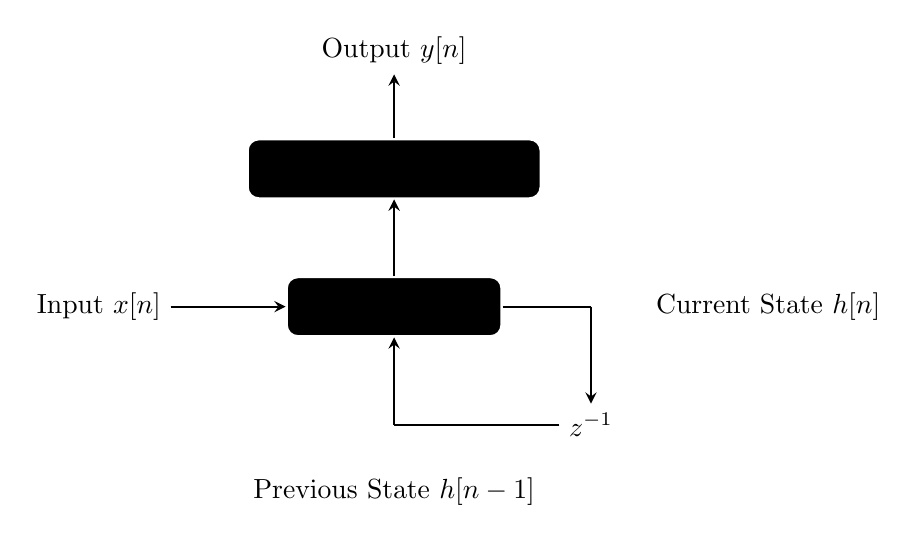
\begin{tikzpicture}[node distance=2.0cm]
            \tikzset{
                mynode/.style = {rectangle, rounded corners, line width=0.8pt, minimum width=2cm, minimum height=0.75cm, text centered, draw=white, fill=black},
                arrow/.style = {thick,->,>=stealth}
            }
            \node (input) {Input $x[n]$};
            \node (rlayer) [mynode, right of=input, xshift=1.75cm] {Recurrent Layer};
            \coordinate[right of=rlayer, xshift=0.5cm] (h0) ;
            \node (h0Label) [right of=h0, xshift=0.25cm] {Current State $h[n]$};
            \node (z1) [rectangle, draw=white, below of=h0, yshift=0.5cm] {$z^{-1}$};
            \coordinate[below of=rlayer, yshift=0.5cm] (h1);
            \node (h1Label) [below of=h1, yshift=1.15cm] {Previous State $h[n-1]$};
    
            \draw [arrow] (input) -- (rlayer);
            \draw [thick] (rlayer) -- (h0);
            \draw [arrow] (h0) -- (z1);
            \draw [thick] (z1) -- (h1);
            \draw [arrow] (h1) -- (rlayer);
    
            \node (dense) [mynode, above of=rlayer, yshift=-0.25cm] {Fully Connected Layer};
            \node (out) [above of=dense, yshift=-0.5cm] {Output $y[n]$};
            \draw [arrow] (rlayer) -- (dense);
            \draw [arrow] (dense) -- (out);
    
        \end{tikzpicture}
    \end{figure}
\end{frame}

\begin{frame}{Recurrent Neural Network}
    Recurrent layer: Gated Recurrent Unit
    \begin{equation}
        z[n] = \sigma(W_z x[n] + U_z h[n-1] + b_z)
    \end{equation}
    \begin{equation}
        r[n] = \sigma(W_r x[n] + U_r h[n-1] + b_r)
    \end{equation}
    \begin{equation}
        c[n] = \tanh(W_c x[n] + r[n] \circ U_c h[n-1] + b_c)
    \end{equation}
    \begin{equation}
        h[n] = z[n] \circ h[n-1] + (1 - z[n]) \circ c[n]
    \end{equation}
\end{frame}

\begin{frame}{Example Circuit: Centaur Gain Stage}
    \begin{figure}
        \centering
        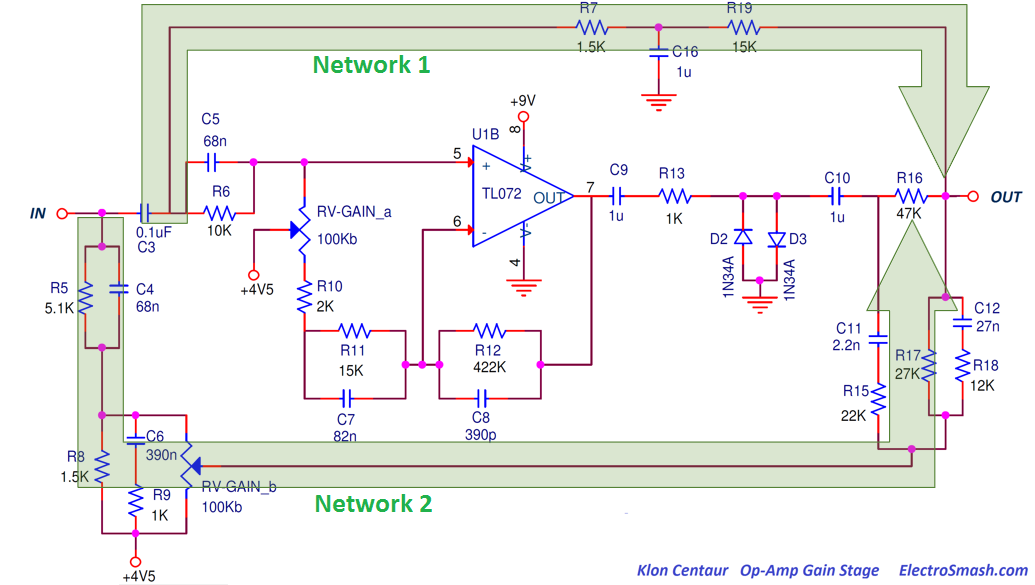
\includegraphics[height=2.5in]{../Paper/Figures/GainStageCircuit.png}
    \end{figure}
\end{frame}

\begin{frame}{Recurrent Neural Network: Training}
    Training Data:
    \begin{itemize}
        \itemsep0em
        \item $\sim 4$ minutes of guitar recordings (direct) at 44.1 kHz
        \item Split into 0.5 second segments
        \item 400 training samples, 25 validation samples
        \item Simulated Klon output using SPICE
        \item 5 positions of ``Gain'' parameter
    \end{itemize}
    \vspace{2ex}
    Loss Function: Error-to-Signal Ratio
    \begin{equation}
        \mathcal{E}_{ESR} = \frac{\sum_{n=0}^{N-1} |y[n] - \hat{y}[n]|^2}{\sum_{n=0}^{N-1} |y[n]|^2}
    \end{equation}
\end{frame}

\begin{frame}{Recurrent Neural Network: Control Parameters}
    In training, we were unable to successfully train a network that
    included the ``Gain'' parameter.\newline\newline
    Instead, we trained 5 independent networks, one for each ``Gain''
    knob position. In the final implementation, we ``fade'' between the
    models in real-time.
\end{frame}
